\chapter{Random Forests}\label{ch:forest}

\begin{remark}{Outline}
In this chapter, we present the well-known family of \textit{Random Forests}
methods. In Section~\ref{sec:4:bias-variance}, we first describe the
bias-variance decomposition of the prediction error and then present, in
Section~\ref{sec:4:ensemble}, how aggregating randomized models through ensembles reduces the prediction
error by decreasing the variance term in this decomposition. In particular, we revisit
Random Forests ant its variants and
study how randomness introduced into the decision tree induction algorithm can
reduce prediction error by decorrelating the decision trees in the ensemble. Finally, the
consistency of forests of randomized trees is explored in
Section~\ref{sec:4:consistency}.
\end{remark}

\section{Bias-variance decomposition}
\label{sec:4:bias-variance}

In section~\ref{sec:2:performance-evaluation}, we defined the generalization
error of a model $\varphi_{\cal L}$ as its expected prediction error
according to some loss function $L$
\begin{equation}
Err(\varphi_{\cal L}) = \mathbb{E}_{X,Y} \{ L(Y, \varphi_{\cal L}(X)) \}.
\end{equation}
Similarly, the expected prediction error of $\varphi_{\cal L}$ at $X=\mathbf{x}$
can be expressed as
\begin{equation}
Err(\varphi_{\cal L}(\mathbf{x})) = \mathbb{E}_{Y|X=\mathbf{x}} \{ L(Y, \varphi_{\cal L}(\mathbf{x})) \}.\label{eqn:4:generalization-error:x}
\end{equation}

In regression, this latter form of the expected prediction error additively
decomposes into bias and variance terms which together constitute a very useful
framework for diagnosing the prediction error of a model. In classification, a
similar decomposition is more difficult to obtain. Yet, as we will see, the
concepts of bias and variance can be transposed in several ways to
classification, thereby providing comparable frameworks for studying the
prediction error of classifiers.

\subsection{Regression error}

In regression, assuming that $L$ is the squared error loss, the expected
prediction error of a model $\varphi_{\cal L}$ at a given point $X=\mathbf{x}$
can be rewritten with respect to the Bayes model $\varphi_B$:
\begin{align}
& Err(\varphi_{\cal L}(\mathbf{x})) \nonumber \\
&= \mathbb{E}_{Y|X=\mathbf{x}} \{ (Y - \varphi_{\cal L}(\mathbf{x}))^2 \} \nonumber \\
&= \mathbb{E}_{Y|X=\mathbf{x}} \{ (Y -\varphi_B(\mathbf{x}) + \varphi_B(\mathbf{x}) - \varphi_{\cal L}(\mathbf{x}))^2 \} \nonumber \\
&= \mathbb{E}_{Y|X=\mathbf{x}} \{ (Y -\varphi_B(\mathbf{x}))^2  \} + \mathbb{E}_{Y|X=\mathbf{x}} \{ (\varphi_B(\mathbf{x}) - \varphi_{\cal L}(\mathbf{x}))^2 \} \nonumber \\
& \quad+ \mathbb{E}_{Y|X=\mathbf{x}} \{ 2 (Y - \varphi_B(\mathbf{x}))(\varphi_B(\mathbf{x}) - \varphi_{\cal L}(\mathbf{x})) \} \nonumber \\
&= \mathbb{E}_{Y|X=\mathbf{x}} \{ (Y -\varphi_B(\mathbf{x}))^2 \} + \mathbb{E}_{Y|X=\mathbf{x}} \{ (\varphi_B(\mathbf{x}) - \varphi_{\cal L}(\mathbf{x}))^2 \} \nonumber \\
&= Err(\varphi_B(\mathbf{x})) +  (\varphi_B(\mathbf{x}) - \varphi_{\cal L}(\mathbf{x}))^2 \label{eqn:4:decomp1}
\end{align}
since $\mathbb{E}_{Y|X=\mathbf{x}} \{ Y - \varphi_B(\mathbf{x}) \} =
\mathbb{E}_{Y|X=\mathbf{x}} \{ Y \} - \varphi_B(\mathbf{x}) = 0$ by definition
of the Bayes model in regression. In this form, the first term in the last
expression of Equation~\ref{eqn:4:decomp1} corresponds to the (irreducible)
residual error  at $X=\mathbf{x}$ while the second term represents the
discrepancy of $\varphi_{\cal L}$ from the Bayes model. The further from the
Bayes model, the more sub-optimal the model and the larger the error.

If we further assume that the learning set ${\cal L}$ is itself a random
variable and that the learning algorithm is deterministic, then the expected
discrepancy with the Bayes model can further be re-expressed in terms of the
average prediction $\mathbb{E}_{\cal L} \{ \varphi_{\cal L}(\mathbf{x}) \}$
over the models learned from all possible learning sets of size $N$:
\begin{align}
& \mathbb{E}_{\cal L} \{ (\varphi_B(\mathbf{x}) - \varphi_{\cal L}(\mathbf{x}))^2 \}\nonumber \\
&= \mathbb{E}_{\cal L} \{ (\varphi_B(\mathbf{x}) - \mathbb{E}_{\cal L} \{ \varphi_{\cal L}(\mathbf{x}) \} + \mathbb{E}_{\cal L} \{ \varphi_{\cal L}(\mathbf{x}) \} - \varphi_{\cal L}(\mathbf{x}))^2 \} \nonumber \\
&= \mathbb{E}_{\cal L} \{ (\varphi_B(\mathbf{x}) - \mathbb{E}_{\cal L} \{ \varphi_{\cal L}(\mathbf{x}) \} )^2 \} + \mathbb{E}_{\cal L} \{ (\mathbb{E}_{\cal L} \{ \varphi_{\cal L}(\mathbf{x}) \} - \varphi_{\cal L}(\mathbf{x}))^2 \} \}\nonumber \\
& \quad+ \mathbb{E}_{\cal L} \{ 2(\varphi_B(\mathbf{x}) - \mathbb{E}_{\cal L} \{ \varphi_{\cal L}(\mathbf{x}) \})(\mathbb{E}_{\cal L} \{ \varphi_{\cal L}(\mathbf{x}) \} - \varphi_{\cal L}(\mathbf{x}))\} \nonumber \\
&= \mathbb{E}_{\cal L} \{ (\varphi_B(\mathbf{x}) - \mathbb{E}_{\cal L} \{ \varphi_{\cal L}(\mathbf{x}) \} )^2 \} + \mathbb{E}_{\cal L} \{ (\mathbb{E}_{\cal L} \{ \varphi_{\cal L}(\mathbf{x}) \} - \varphi_{\cal L}(\mathbf{x}))^2 \} \}\nonumber \\
&= (\varphi_B(\mathbf{x}) - \mathbb{E}_{\cal L} \{ \varphi_{\cal L}(\mathbf{x}) \} )^2 + \mathbb{E}_{\cal L} \{ (\mathbb{E}_{\cal L} \{ \varphi_{\cal L}(\mathbf{x}) \} - \varphi_{\cal L}(\mathbf{x}))^2 \}
\end{align}
since $\mathbb{E}_{\cal L}\{ \mathbb{E}_{\cal L} \{ \varphi_{\cal
L}(\mathbf{x}) \} - \varphi_{\cal L}(\mathbf{x}) \} =  \mathbb{E}_{\cal L} \{
\varphi_{\cal L}(\mathbf{x}) \} -  \mathbb{E}_{\cal L} \{ \varphi_{\cal
L}(\mathbf{x}) \} = 0$. In summary, the expected generalization error additively
decomposes as formulated in Theorem~\ref{thm:bias-variance}.

\begin{theorem}\label{thm:bias-variance}
The bias-variance decomposition of the expected generalization error
$\mathbb{E}_{\cal L} \{ Err(\varphi_{\cal L}(\mathbf{x})) \}$ at $X=\mathbf{x}$
is:
\begin{equation}
\mathbb{E}_{\cal L} \{ Err(\varphi_{\cal L}(\mathbf{x})) \} = \text{noise}(\mathbf{x}) + \text{bias}^2(\mathbf{x}) + \text{var}(\mathbf{x})
\end{equation}
where
\begin{align}
\text{noise}(\mathbf{x}) &= Err(\varphi_B(\mathbf{x})) \\
\text{bias}^2(\mathbf{x}) &= (\varphi_B(\mathbf{x}) - \mathbb{E}_{\cal L} \{ \varphi_{\cal L}(\mathbf{x}) \} )^2 \\
\text{var}(\mathbf{x}) &= \mathbb{E}_{\cal L} \{ (\mathbb{E}_{\cal L} \{ \varphi_{\cal L}(\mathbf{x}) \} - \varphi_{\cal L}(\mathbf{x}))^2 \}
\end{align}
\end{theorem}

This bias-variance decomposition of the generalization error is due to
\citet{geman:1992} and was first proposed in the context of neural networks.
The first term, $\text{noise}(\mathbf{x})$, is the residual error. It is
entirely independent of both the learning algorithm and the learning set and
provides for any model a theoretical lower bound on its generalization error.
The second term, $\text{bias}^2(\mathbf{x})$, measures the discrepancy between
the average prediction and the prediction of the Bayes model. Finally, the
third term, $\text{var}(\mathbf{x})$, measures the variability of the
predictions at $X=\mathbf{x}$ over the models learned from all possible
learning sets. All three terms are illustrated in Figure~\ref{fig:bias-variance}
for a toy regression problem. Both $\text{noise}(\mathbf{x})$ and
$\text{var}(\mathbf{x})$ measures the spread of the two densities while
$\text{bias}^2(\mathbf{x})$ is the distance between their means.

\begin{figure}
    \centering
    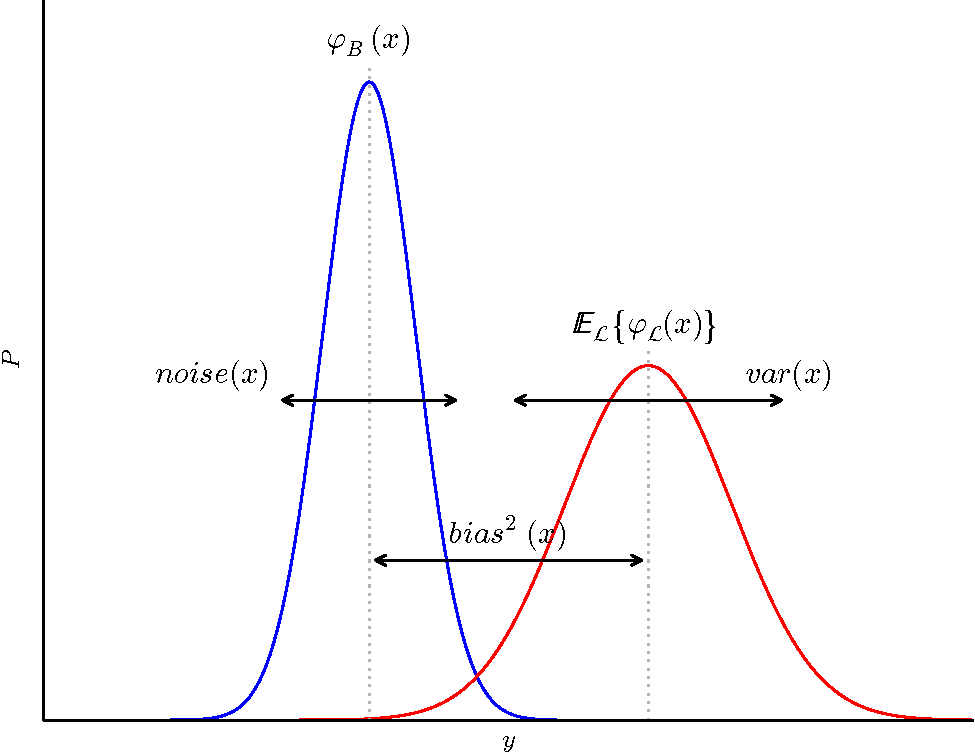
\includegraphics[width=0.9\textwidth]{figures/ch4_bias_variance.pdf}
    \caption{Residual error, bias and variance at $X=\mathbf{x}$. (Figure inspired from \citep{geurts:2002}.)}
    \label{fig:bias-variance}
\end{figure}

As a typical example, the bias-variance decomposition framework can be used as
a tool for diagnosing underfitting and overfitting (as previously introduced in
Section \ref{sec:2:model-selection}). The upper plots in
Figure~\ref{fig:overfitting} illustrate in light red predictions $\varphi_{\cal
L}(\mathbf{x})$ for polynomials of degree $1$, $5$ and $15$ learned over random
learning sets ${\cal L}$ sampled from a noisy cosinus function. Predictions
$\mathbb{E}_{\cal L} \{ \varphi_{\cal L}(\mathbf{x}) \}$ of the average model
are represented by the thick red lines. Predictions for the model learned over
the learning set represented by the blue dots are represented in gray.
Predictions of the Bayes model are shown in blue and coincide with the unnoised
cosinus function that defines the regression problem. The lower plots in the
figure illustrate the bias-variance decomposition of the expected
generalization error of the polynomials.

\begin{figure}
    \hspace{-0.75cm}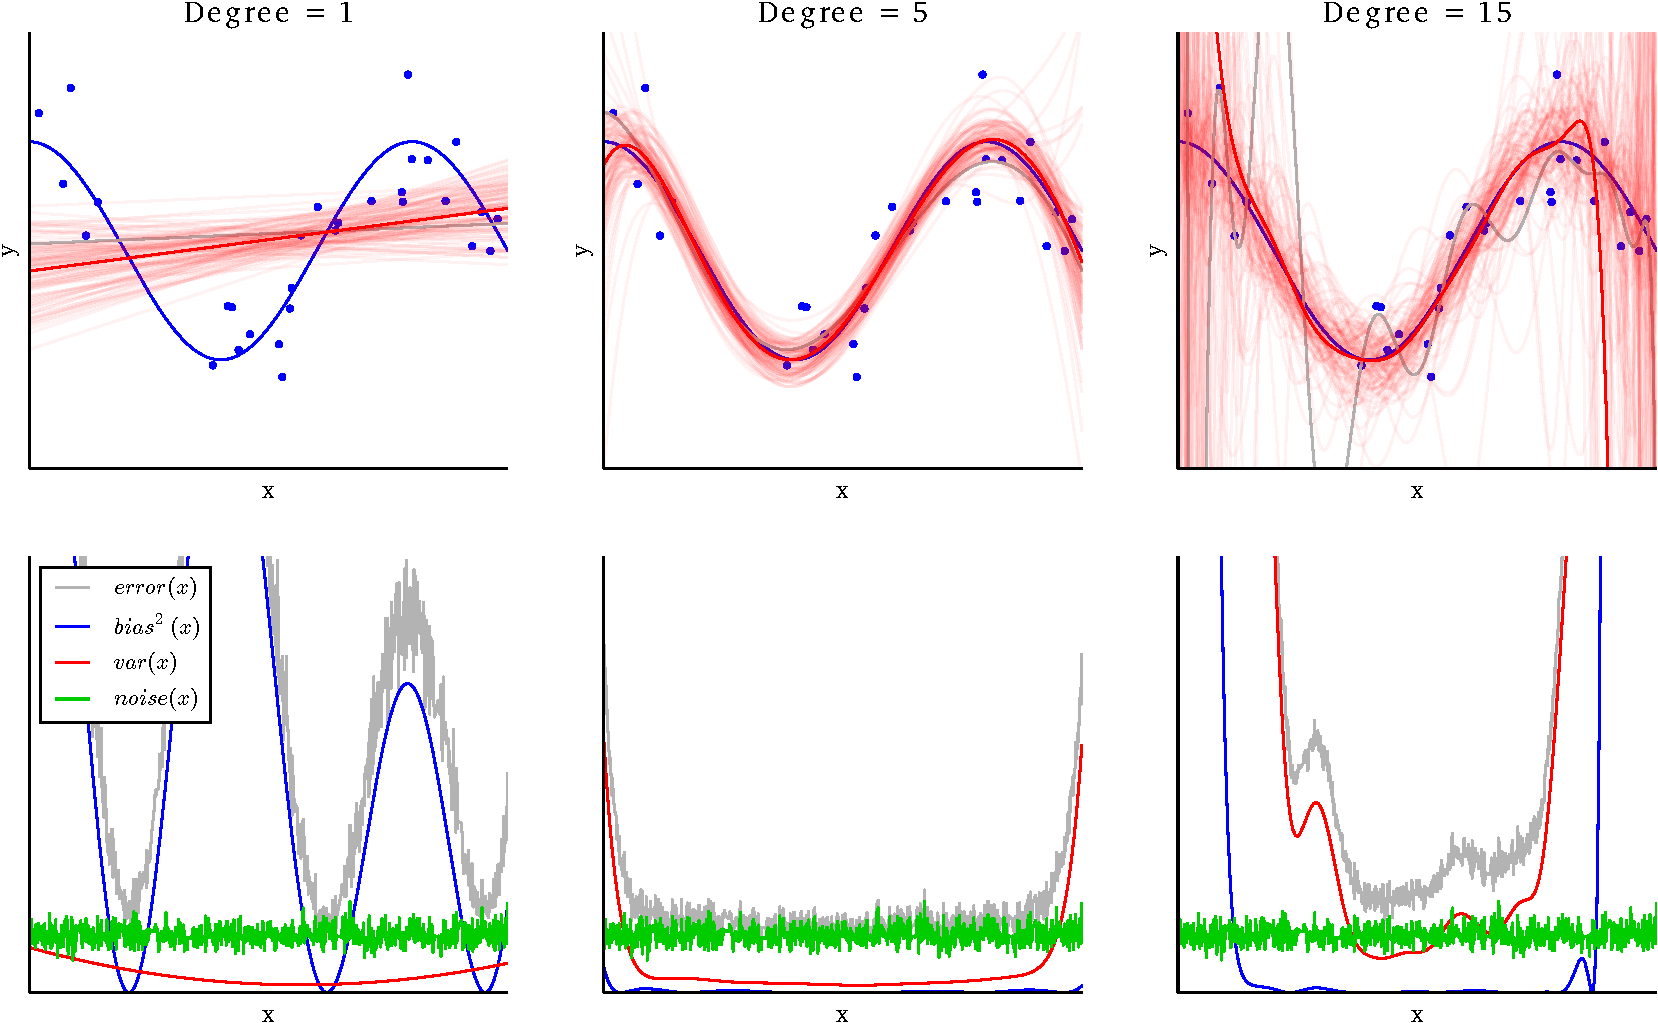
\includegraphics[width=1.1\textwidth]{figures/ch4_overfitting.pdf}
    \caption{Bias-variance decomposition of the expected generalization error for polynomials of degree $1$, $5$ and $15$.}
    \label{fig:overfitting}
\end{figure}

Clearly, polynomials of degree $1$ (left) suffer from underfitting. In terms of
bias and variance, this translates into low variance but high bias as shown in
the lower left plot of Figure~\ref{fig:overfitting}. Indeed, due to the low
degree of the polynomials (i.e., due to the low model complexity), the
resulting models are almost all identical and  the variability of the
predictions from one model to another is therefore quite low. Also, because of
low complexity, none of them really fits the trend of the training points, even
approximately, which implies that the average model is far from approximating
the Bayes model. This results in high bias. On the other hand, polynomials of
degree $15$ (right) suffer from overfitting. In terms of bias and variance, the
situation is the opposite. Predictions have low bias but high variance, as
shown in the lower right plot of Figure~\ref{fig:overfitting}. The variability
of the predictions is large because the high degree of the polynomials (i.e.,
the high model complexity) captures noise in the learning set. Indeed,
compare the gray line with the blue dots -- they almost all intersect. Put
otherwise, small changes in the learning set result in large changes in the
obtained model and therefore in its predictions. By contrast, the average model is
now quite close from the Bayes model, which results in low bias\footnote{Note
however the Gibbs-like phenomenon resulting in both high variance and high bias
at the boundaries of ${\cal X}$.}. Finally, polynomials of degree $5$ (middle)
are neither too simple nor too complex. In terms of bias and variance, the
trade-off is well-balanced between the two extreme situations. Bias and
variance are neither too low nor too large.

\subsection{Classification error}

\todo{}


\section{Ensembles of randomized trees}
\label{sec:4:ensemble}

\subsection{Bias and variance of a randomized tree}

% bias variance of randomized

\subsection{Bias and variance of an ensemble of randomized trees}

% bias variance of ensemble of randomized
    % Aggregation
    % > consensus vote
    % > average probability (Hastie, 283+)
    % > average output values

% discussion on the correlation coefficient + increase of bias

% RF do not overfit (theorem 2.3)

\subsection{Random Forests}

% random forests algorithms
    % - Bagging
    % - Random features (Kwok & carter (1990), dietterich 1998 (see rf), breiman)
    % - Random thresholds (geurts)
    % - +other kinds of forests (see state-of-the-art in geurts)
    % => discuter sur un exemple les aspects stat/comput/repres
    % Ex: correlation coeff example

% Issues tackled by ensemble
%   Ensemble methods in ML, Dietterich
%   - stat
%   - computational
%   - representational

% OOB estimates

\section{Consistency}
\label{sec:4:consistency}

    % > Mise au point
    % > Preuve de consistence des extra-trees?
